 %% abtex2-modelo-trabalho-academico.tex, v-1.9.2 laurocesar

%% Copyright 2012-2014 by abnTeX2 group at http://abntex2.googlecode.com/ 
%%
%% This work may be distributed and/or modified under the
%% conditions of the LaTeX Project Public License, either version 1.3
%% of this license or (at your option) any later version.
%% The latest version of this license is in
%%   http://www.latex-project.org/lppl.txt
%% and version 1.3 or later is part of all distributions of LaTeX
%% version 2005/12/01 or later.
%%
%% This work has the LPPL maintenance status `maintained'.
%% 
%% The Current Maintainer of this work is the abnTeX2 team, led
%% by Lauro César Araujo. Further information are available on 
%% http://abntex2.googlecode.com/
%%
%% This work consists of the files abntex2-modelo-trabalho-academico.tex,
%% abntex2-modelo-include-comandos and abntex2-modelo-references.bib
%%

% ------------------------------------------------------------------------
% ------------------------------------------------------------------------
% abnTeX2: Modelo de Trabalho Academico (tese de doutorado, dissertacao de
% mestrado e trabalhos monograficos em geral) em conformidade com 
% ABNT NBR 14724:2011: Informacao e documentacao - Trabalhos academicos -
% Apresentacao
% ------------------------------------------------------------------------
% ------------------------------------------------------------------------

\documentclass[
	% -- opções da classe memoir --
	12pt,				% tamanho da fonte
	openright,			% capítulos começam em pág ímpar (insere página vazia caso preciso)
	twoside,			% para impressão em verso e anverso. Oposto a oneside
	a4paper,			% tamanho do papel. 
	% -- opções da classe abntex2 --
	%chapter=TITLE,		% títulos de capítulos convertidos em letras maiúsculas
	%section=TITLE,		% títulos de seções convertidos em letras maiúsculas
	%subsection=TITLE,	% títulos de subseções convertidos em letras maiúsculas
	%subsubsection=TITLE,% títulos de subsubseções convertidos em letras maiúsculas
	% -- opções do pacote babel --
	english,			% idioma adicional para hifenização
	french,				% idioma adicional para hifenização
	spanish,			% idioma adicional para hifenização
	brazil				% o último idioma é o principal do documento
	]{abntex2}
%https://code.google.com/p/abntex2/wiki/Texmaker
% ---
% Pacotes básicos 
% ---
\usepackage{lmodern}			% Usa a fonte Latin Modern			
\usepackage[T1]{fontenc}		% Selecao de codigos de fonte.
\usepackage[utf8]{inputenc}		% Codificacao do documento (conversão automática dos acentos)
\usepackage{lastpage}			% Usado pela Ficha catalográfica
\usepackage{indentfirst}		% Indenta o primeiro parágrafo de cada seção.
\usepackage{color}				% Controle das cores
\usepackage{graphicx}			% Inclusão de gráficos
\usepackage{microtype} 			% para melhorias de justificação
\usepackage{url}
\usepackage[table,xcdraw]{xcolor}
\usepackage{enumitem}

% ---
		
% ---
% Pacotes adicionais, usados apenas no âmbito do Modelo Canônico do abnteX2
% ---
\usepackage{lipsum}				% para geração de dummy text
% ---

% ---
% Pacotes de citações
% ---
\usepackage[brazilian,hyperpageref]{backref}	 % Paginas com as citações na bibl
\usepackage[alf]{abntex2cite}	% Citações padrão ABNT

%%%%%%%%%%% syntax highlight %%%%%%%%%%%%%%%%%%%%%%%%%%%%%%%%%%%%%%%%%%%%%%%%%%%%%


\usepackage{listings}
\definecolor{maroon}{rgb}{0.5,0,0}
\definecolor{darkgreen}{rgb}{0,0.5,0}
\definecolor{deepblue}{rgb}{0,0,0.5}
\definecolor{deepred}{rgb}{0.6,0,0}
\definecolor{purple}{rgb}{0.5,0,0.5}
\definecolor{deepgreen}{rgb}{0,0.5,0}








%%%%%%%%%%%%%%%%%%%%%%%%%%%%%%%%%%%%%%%%%%%%%%%%%%%%%%% 


% --- 
% CONFIGURAÇÕES DE PACOTES
% --- 

% ---
% Configurações do pacote backref
% Usado sem a opção hyperpageref de backref
\renewcommand{\backrefpagesname}{Citado na(s) página(s):~}
% Texto padrão antes do número das páginas
\renewcommand{\backref}{}
% Define os textos da citação
\renewcommand*{\backrefalt}[4]{
	\ifcase #1 %
		Nenhuma citação no texto.%
	\or
		Citado na página #2.%
	\else
		Citado #1 vezes nas páginas #2.%
	\fi}%
% ---

% ---
% Informações de dados para CAPA e FOLHA DE ROSTO
% ---
\titulo{Luteria Composicional de algoritmos pós-tonais }
\autor{Guilherme Rafael Soares}
%\local{Brasil}
\data{10 de julho de 2014, v0.6-Qualificação}
\orientador{Prof. Dr. Daniel Quaranta}
%\coorientador{Equipe \abnTeX}
\instituicao{%
  UFJF - Universidade Federal de Juiz de Fora
  \par
  Instituto de Artes e Design
  \par
  Programa de Pós-Graduação em Artes, Cultura e Linguagens}
\tipotrabalho{Tese (Mestrado)}
% O preambulo deve conter o tipo do trabalho, o objetivo, 
% o nome da instituição e a área de concentração 
\preambulo{Prévia da dissertação para a banca de qualificação para o Mestrado em Arte, Cultura e Linguagens do IAD-UFJF.}
% ---


% ---
% Configurações de aparência do PDF final

% alterando o aspecto da cor azul
\definecolor{blue}{RGB}{41,5,195}

% informações do PDF
\makeatletter
\hypersetup{
     	%pagebackref=true,
		pdftitle={\@title}, 
		pdfauthor={\@author},
    	pdfsubject={\imprimirpreambulo},
	    pdfcreator={LaTeX with abnTeX2},
		pdfkeywords={abnt}{latex}{abntex}{abntex2}{trabalho acadêmico}, 
		colorlinks=true,       		% false: boxed links; true: colored links
    	linkcolor=blue,          	% color of internal links
    	citecolor=blue,        		% color of links to bibliography
    	filecolor=magenta,      		% color of file links
		urlcolor=blue,
		bookmarksdepth=4
}
\makeatother
% --- 

% --- 
% Espaçamentos entre linhas e parágrafos 
% --- 

% O tamanho do parágrafo é dado por:
\setlength{\parindent}{1.3cm}

% Controle do espaçamento entre um parágrafo e outro:
\setlength{\parskip}{0.2cm}  % tente também \onelineskip

% ---
% compila o indice
% ---
\makeindex
% ---

% ----
% Início do documento
% ----
\begin{document}

% Retira espaço extra obsoleto entre as frases.
\frenchspacing 

% ----------------------------------------------------------
% ELEMENTOS PRÉ-TEXTUAIS
% ----------------------------------------------------------
% \pretextual

% ---
% Capa
% ---
\imprimircapa
% ---


% ---
% Folha de rosto
% (o * indica que haverá a ficha bibliográfica)
% ---
\imprimirfolhaderosto*
% ---

% ---
% Inserir a ficha bibliografica
% ---

% Isto é um exemplo de Ficha Catalográfica, ou ``Dados internacionais de
% catalogação-na-publicação''. Você pode utilizar este modelo como referência. 
% Porém, provavelmente a biblioteca da sua universidade lhe fornecerá um PDF
% com a ficha catalográfica definitiva após a defesa do trabalho. Quando estiver
% com o documento, salve-o como PDF no diretório do seu projeto e substitua todo
% o conteúdo de implementação deste arquivo pelo comando abaixo:
%
% \begin{fichacatalografica}
%     \includepdf{fig_ficha_catalografica.pdf}
% \end{fichacatalografica}
\begin{fichacatalografica}
	\vspace*{\fill}					% Posição vertical
	\hrule							% Linha horizontal
	\begin{center}					% Minipage Centralizado
	\begin{minipage}[c]{12.5cm}		% Largura
	
	\imprimirautor
	
	\hspace{0.5cm} \imprimirtitulo  / \imprimirautor. --
	\imprimirlocal, \imprimirdata-
	
	\hspace{0.5cm} \pageref{LastPage} p. : il. (algumas color.) ; 30 cm.\\
	
	\hspace{0.5cm} \imprimirorientadorRotulo~\imprimirorientador\\
	
	\hspace{0.5cm}
	\parbox[t]{\textwidth}{\imprimirtipotrabalho~--~\imprimirinstituicao,
	\imprimirdata.}\\
	
	\hspace{0.5cm}
		1. Palavra-chave1.
		2. Palavra-chave2.
		I. Orientador: Prof. Dr. Daniel Quaranta
		II. UFJF - Universidade Federal de Juiz de Fora.
		III. Instituto de Artes e Design
		IV. \imprimirtitulo \\ 			
	
	\hspace{8.75cm} CDU 02:141:005.7\\
	
	\end{minipage}
	\end{center}
	\hrule
\end{fichacatalografica}
% ---

% ---
% Inserir errata
% ---
%\begin{errata}
%Elemento opcional da \citeonline[4.2.1.2]{NBR14724:2011}. Exemplo:
%
%\vspace{\onelineskip}
%
%FERRIGNO, C. R. A. \textbf{Tratamento de neoplasias ósseas apendiculares com
%reimplantação de enxerto ósseo autólogo autoclavado associado ao plasma
%rico em plaquetas}: estudo crítico na cirurgia de preservação de membro em
%cães. 2011. 128 f. Tese (Livre-Docência) - Faculdade de Medicina Veterinária e
%Zootecnia, Universidade de São Paulo, São Paulo, 2011.
%
%\begin{table}[htb]
%\center
%\footnotesize
%\begin{tabular}{|p{1.4cm}|p{1cm}|p{3cm}|p{3cm}|}
%  \hline
%   \textbf{Folha} & \textbf{Linha}  & \textbf{Onde se lê}  & \textbf{Leia-se}  \\
%    \hline
%    1 & 10 & auto-conclavo & autoconclavo\\
%   \hline
%\end{tabular}
%\end{table}

%\end{errata}
% ---

% ---
% Inserir folha de aprovação
% ---

% Isto é um exemplo de Folha de aprovação, elemento obrigatório da NBR
% 14724/2011 (seção 4.2.1.3). Você pode utilizar este modelo até a aprovação
% do trabalho. Após isso, substitua todo o conteúdo deste arquivo por uma
% imagem da página assinada pela banca com o comando abaixo:
%
% \includepdf{folhadeaprovacao_final.pdf}
%
\begin{folhadeaprovacao}

  \begin{center}
    {\ABNTEXchapterfont\large\imprimirautor}

    \vspace*{\fill}\vspace*{\fill}
    \begin{center}
      \ABNTEXchapterfont\bfseries\Large\imprimirtitulo
    \end{center}
    \vspace*{\fill}
    
    \hspace{.45\textwidth}
    \begin{minipage}{.5\textwidth}
        \imprimirpreambulo
    \end{minipage}%
    \vspace*{\fill}
   \end{center}
        
   Trabalho aprovado \imprimirlocal, 13 de fevereiro de 2015:

   \assinatura{\textbf{\imprimirorientador} \\ Orientador} 
   \assinatura{\textbf{Professor} \\ Convidado 1}
   \assinatura{\textbf{Professor} \\ Convidado 2}
   %\assinatura{\textbf{Professor} \\ Convidado 3}
   %\assinatura{\textbf{Professor} \\ Convidado 4}
      
   \begin{center}
    \vspace*{0.5cm}
    {\large\imprimirlocal}
    \par
    {\large\imprimirdata}
    \vspace*{1cm}
  \end{center}
  
\end{folhadeaprovacao}
% ---

% ---
% Dedicatória
% ---
%\begin{dedicatoria}
%   \vspace*{\fill}
%   \centering
%   \noindent
%   \textit{ Este trabalho é dedicado às crianças adultas que,\\
%   quando pequenas, sonharam em se tornar cientistas.} \vspace*{\fill}
%\end{dedicatoria}
% ---

% ---
% Agradecimentos
% ---
%\begin{agradecimentos}

%A você...\footnote{...principalmente pela atenção até nas notas de rodapé.}



%\end{agradecimentos}
% ---

% ---
% Epígrafe cortazar
% ---
%\begin{epigrafe}
%    \vspace*{\fill}
%	\begin{flushright}
%		\textit{``Quantas vezes me pergunto se isto não é mais do que escrita, numa época em que corremos para o %engano entre equações infalíveis e máquinas de conformismos? Mas perguntar se saberemos encontrar o outro lado do %hábito ou se mais vale se deixar levar pela sua alegre cibernética, não será mais uma vez literatura? Revolta, %conformismo, angústia, alimentos terrestres, todas as dicotomias: o Yin e o Yang, a contemplação (...) e, %finalmente; um encolher de ombros, a paz, o parafuso foi a paz, ninguém podia passar pela rua sem olhar de soslaio %para o parafuso e sentir que ele era a paz. \cite{cortazar1963} }
%	\end{flushright}
%\end{epigrafe}



% ---

% ---
% RESUMOS
% ---

% resumo em português

\setlength{\absparsep}{18pt} % ajusta o espaçamento dos parágrafos do resumo



\begin{resumo}


Esta pesquisa visa problematizar e sistematizar um catálogo de experimentos constituído de pequenas peças musicais e seus algoritmos geradores, objetivando a construção de uma biblioteca de objetos para composição assistida por computador que gere partituras baseadas em regras quantitativas extraídas de análises musicais.

Formalizamos tais aspectos através de um estudo comparado de dois paradigmas de análise musical: \textit{"A Teoria Gerativa da Música Tonal"}\cite{lerdahl1983generative} com algumas de suas continuidades  \cite{lerdahl2009genesis,temperley2001cognition} e a \textit{"Teoria de grupos das classes de alturas"\ (ou "Pitch Class Set Theory")}  \cite{forte1973structure,straus2004}.

Os procedimentos são demonstrados a partir de aspectos singulares de algumas peças da suíte Mikrokosmos do compositor Béla Bartók, gerando composições algorítmicas a partir das regras observadas. Este repertório foi escolhido devido a seu reconhecido contexto como composições pianísticas e pedagógicas situadas nas fronteiras da pós-tonalidade. 

Apontamos as limitações encontradas na aplicação dos paradigmas analíticos adotados aqui no contexto da suíte de peças escolhidas e suas derivações composicionais.

Detalhamos questões computacionais para esta implementação e deixamos um legado de código aberto para continuidades possíveis deste trabalho.


 \textbf{Palavras-chaves}: Música algorítmica. Pós-tonalismo. Teoria dos conjuntos. Pitch class theory. Luteria. Composição assistida por computador. Cibernética. Software livre. Cognição musical. Teoria Gerativa da Música Tonal. Mikrokosmos. Arte Sonora.
\end{resumo}

%%%%%%%%%% traduçoes resumo
\begin{comment}
% resumo em inglês
\begin{resumo}[Abstract]
 \begin{otherlanguage*}{english}
   This is the english abstract.

   \vspace{\onelineskip}
 
   \noindent 
   \textbf{Key-words}: latex. abntex. text editoration.
 \end{otherlanguage*}
\end{resumo}

% resumo em francês 
\begin{resumo}[Résumé]
 \begin{otherlanguage*}{french}
    Il s'agit d'un résumé en français.
 
   \textbf{Mots-clés}: latex. abntex. publication de textes.
 \end{otherlanguage*}
\end{resumo}

% resumo em espanhol
\begin{resumo}[Resumen]
 \begin{otherlanguage*}{spanish}
   Este es el resumen en español.
  
   \textbf{Palabras clave}: latex. abntex. publicación de textos.
 \end{otherlanguage*}
\end{resumo}
% ---
\end{comment}


% ---
% inserir lista de ilustrações
% ---
\pdfbookmark[0]{\listfigurename}{lof}
\listoffigures*
\cleardoublepage
% ---

% ---
% inserir lista de tabelas
% ---
%\pdfbookmark[0]{\listtablename}{lot}
%\listoftables*
%\cleardoublepage
% ---

% ---
% inserir lista de abreviaturas e siglas
% ---
\begin{siglas}
  \item[GTTM] \textit{Generative Theory of Tonal Music}\footnote{ "Teoria Gerativa da Música Tonal"      \cite{lerdahl1983generative} }
  \item[TPS] \textit{Tonal Pitch Space}\footnote{ "Espaço das Alturas Tonais"\cite{lerdahl1988tps} }
  \item[CBMS] \textit{Cognition of Basic Musical Structures}\footnote{ "Cognição das Estruturas Musicais Básicas"\cite{temperley2001cognition} }
  \item[OM] \textit{Open Music}\footnote{ \url{http://repmus.ircam.fr/openmusic/home}. Acessado em 10 de julho de 2014. }
  \item[PD] \textit{Pure Data}\footnote{ \url{http://puredata.info}. Acessado em 10 de julho de 2014. }
\end{siglas}
% ---

% ---
% inserir lista de símbolos
% ---
%\begin{simbolos}
%  \item[$ \Gamma $] Letra grega Gama
%  \item[$ \Lambda $] Lambda
%  \item[$ \zeta $] Letra grega minúscula zeta
%  \item[$ \in $] Pertence
%\end{simbolos}
% ---

% ---
% inserir o sumario
% ---
\pdfbookmark[0]{\contentsname}{toc}
\tableofcontents*
\cleardoublepage
% ---

%
%
%
%
%
%
%
% ----------------------------------------------------------
% ELEMENTOS TEXTUAIS
% ----------------------------------------------------------
\textual

% ----------------------------------------------------------
% Introdução (exemplo de capítulo sem numeração, mas presente no Sumário)
% ----------------------------------------------------------

Este trabalho inicia-se com 

\chapter*[Introdução]{Introdução}
\addcontentsline{toc}{chapter}{Introdução}

lalalala


\part{Percurso pela Analise Musical }


\chapter{Percurso pela Analise Musical}

Prioridade na descrição de métodos da biblioteca music21

Opção por Python http://spectrum.ieee.org/computing/software/top-10-programming-languages 


\section{Análise musical para regras gerativas }

dfdkjsfsk


\section{Musicologia Assistida por computador}



Iniciamos esta pesquisa buscando entender como o percurso que as formalizações computacionais de elementos básicos da cognição musical permitiram o atual estágio da musicologia assistida por computador. Trabalhos como as primeiras tentativas de definir gramáticas computáveis de Curtis \citeonline{roads1979grammars}, a formalização de uma gramática gerativa da música tonal proposta por \citeonline{lerdahl1983generative} e derivações que geraram implementações computacionais como as pesquisas de \citeonline{temperley2001cognition} e \citeonline{huron2006sweet} nos interessaram e pareceram a princípio essenciais como base para o entendimento de algoritmos de segmentação de estruturas musicais observáveis em partituras e arquivos de corpus derivados de instruções composicionais simbólicas.

No entanto percebemos no decorrer de nosso aprofundamento nesta bibliografia específica que descrever todo seu escopo em profundidade e abrangência apresentava duas questões essenciais de prioridades para o presente trabalho, considerndo o caso da teoria pós-tonal almejada aqui e em especial para as particularidades presentes na música de Bela Bartók que pudessem interessar como singularidade composicional: 


1) As abordagens generalistas dos problemas quantizáveis de expectativa musical com base em pesquisas sobre cognição e fruição da linguagem tonal, uma música de tradição clássica e romântica ocidental, repertório referido como "de prática comum"\footnote{c.f. temprley} e seus problemas de ordem métrica, rítmica, melódica, harmônica e prolongacional\footnote{tradição shenkeriana} quase sempre tangenciam a música que interessa na presente pesquisa como uma exceção especializada das regras gerais, o que nos chamou a atenção para quais seriam as alternativas a uma abordagem que partisse de outros princípios. 

Encontramos então na literatura específica das análises do repertório bartokiano e na literatura que funda algums nomenclaturas da análise pós-tonal um ponto de partida mais objetivo: organização de sonoridades por novos critérios de organização intervalar, casos de observação de simetrias, ciclos transposições e transformações destes materiais e a busca por descrições de outras lógicas de encadeamento deste material intervalar e sua relação com as percepções mais básicas que ainda operam o lstro de expectativa tonal

2) Dado o período de quase quatro décadas das primeiras implementações destes algoritmos de segmentação musical temos atualmente um cenário bastante amplo para testar muitas destas teorias e buscar compreende-las a mperlepartir de uma experiência prática. Alguns dos algoritmos implementados por Temperley, Huron e pesquisas similares podem ser experimentados com a biblioteca python Music21, que foi usada em nossos estudos de caso. Consideramos esta uma melhor estratégia fazer as digressões sobre as origens destes algoritmos a partir destas implementações, seus usos e limitações na presente pesquisa, portanto.




\chapter{Apontamentos Bartokianos}

\section{Panorama básico sobre analise bartokiana}

Malcom Gillies propõe em seu artigo \textit{"Bartók Analysis and Authenticity"}\cite{gillies1995bartok}\ um panorama dos problemas e lugares comum nas análises de Bartók, apontando alguns critérios para o que poderiam ao menos garantir a \textit{"autenticidade"}\ entre as diversas correntes analíticas encontradas até então, já que estas são tão diversas que podem facilmente fechar-se em suas próprias contradições. 

Gillies inicia a reflexão destacando o notável desafio em argumentarmos qualquer esboço totalizante que sustente a unidade entre os níveis das \textit{ "micro"}\ e \textit{"macro"}\ estruturas extraídas da vasta gama de análises disponíveis sobre Bartók até aquele momento.

As \textit{ "micro"}\ estruturas seriam as destacadas com apontamentos de interações entre ciclos e simetrias intervalares, pelas estratégias polimodais que libertam as melodias do tonalismo e criam temas que tornam-se por transposição complementarmente um total cromático, e em geral quaisquer relações que definam contextos que dão uma identidade de sonoridade a fragmentos ainda descontextualizados de uma suposta função num todo. 

As \textit{"macro"}\ estruturas seriam planos gerais que sejam definidos pelas estruturas notáveis de obras inteiras ou conjuntos de obras como unidade - por exemplo questões sobre o encadeamento de secções por alguma estrutura de prolongamento de expectativa, localização de alguma sugestão ambígua de tonalidade e modalismo nos encadeamentos dos grandes blocos, medidas gerais de um plano de equilíbrio das partes com eixos geométricos inspirados na secção áurea ou mesmo a referência a formas mais tradicionais como a sonata.

Gilles propõe antes de tudo, para ater-se a uma questão primordial sobre o que pode ser definido como consenso e o que pode ser considerado idiossincrático, a seguinte classificação por uma diferença de abordagem das análises: \textit{análises "autênticas"}, \textit{"semi-autênticas"} ou \textit{"não-autênticas"}, sem que nisso haja algum sentido depreciativo, mas apenas como critério para entender que este território pode ir de um historicismo de lastro documentado até alguma teoria mais inventiva e sem necessidade de comprovação da consciência do compositor sobre estes aspectos, uma teoria comprometida mais com a inspiração de processos criativos derivados.

\pagebreak
A \textit{\textbf{"autenticidade"}} seria sobretudo definida por critérios de alguma formalização sustentada por vestígios deixados pelo próprio Bartók, como na compilação \textit{"Bela Bartók Essays"}\cite{bartok1993bela}. Considera também nesta categoria as pesquisas que a partir dos registros da pesquisa etnomusicológica de Bartók busca fontes originais de estudos dos aspectos folk de seu trabalho. Entram aqui também as analises que tomam em consideração as performances registradas em áudio que foram executadas pelo próprio Bartók ou supervisionadas por ele, para destacar aspectos complementares aos escritos e partituras originais. 

Uma \textit{\textbf{"semi-autenticidade"}} seria definida a partir de analogias entre influências de outros compositores ou contextos de gênero presentes na obra de Bartók, como por exemplo discurso sobre a influência do drama em sua ópera ou a localização de traços ou citações paródicas por influência de outros compositores em suas peças. Dada autenticidade da analogia portanto, a preocupação com a legitimidade ficaria deslocada para aspectos externos a obra de Bartók.

Já a \textit{\textbf{"não-autenticidade"}} comportaria os estudos da música de Bartók como fonte para apontamentos arbitrários para demonstrações de harmonia funcional, contraponto, análise shenkeriana ou análise pós-tonal por grupos de classes de alturas. Gillies situa também aqui algumas análises de Bartók que tomam caminhos mais especulativos e originais como as análises de proporção geométrica e simetria propostas por Ern{\H{o}} \citeonline{lendvai1971bela}  ou o escrutínio de relações celulares e suas transformações entre ciclos intervalares, rotações motívicas, coleções modais ou não-diatônicas presentes em trabalhos como o de Elliot \citeonline{antokoletz1984music}. 

Em nossa pequena amostra de abordagens seguimos muito mais por este percurso mais descontextualizado e autoral de analistas que destacaram alguns traços estruturais na musica de Bartók e seus Mikrokosmos. Não temos ainda a ambição de esgotar ou mesmo de argumentar uma hierarquia de importâncias "autênticas"\ destes traços em sua obra como um todo ou na consistência geral de seu estilo. Nossa intenção aqui foi apontar limites e possibilidades para uma automação algorítmica de manipulação de transformações sugeridas nestas análises e abrir caminho para uma musica generativa inspirada nestes procedimentos.

\section{Sistema de Eixos de Lendvai}

Ern{\H{o}} \citeonline[p. 08]{lendvai1971bela} organiza uma visão geral de uma transformação de conceitos de harmonia tonal funcional pelo prisma do que chama de \textit{"sistema de eixos"}\footnote{axis system}\ de Bartók. \pagebreak

Estes apontamentos são organizados a partir de seis pontos chave: \textit{\textbf{a)}Afinidades funcionais entre quarto e quinto graus,\textbf{ b)}A relação relativa entre grau maior e menor, \textbf{c)}as especificidades da coleção acústica (overtone), \textbf{d)}os papeis das notas sensíveis , \textbf{e)}das tensões contrapostas de subdominante e dominante, \textbf{f)}a dualidade entre os princípios de tonalidade e distância.}

\subsection{Afinidades funcionais entre quarto e quinto graus}

Partindo da consideração do ciclo das quintas como um esquema rotativo de transformação que possui as forças \textit{subdominante<-tonica->dominante} em cada um dos passos de 30 graus, lembremos que girando da \textit{esquerda para direita} temos sempre uma relação onde \textit{a dominante como nova tônica terá a tônica anterior como subdominante} e girando \textit{da direita a esquerda} teremos uma nova tônica que possui \textit{a tônica anterior como dominante}. 

\citeonline[ p.3]{lendvai1971bela} propõe a partir disso a observação do uso das relações entre os quatro pólos dos três eixos possíveis de transposição que agrupam as doze alturas cromáticas em três eixos de quatro notas. 

\begin{figure}[!h]
	\caption{\label{fig_grafico}Os três eixos das transposições possíveis para a rotação "subdominante-tônica-dominante" .}
	\begin{center}
	    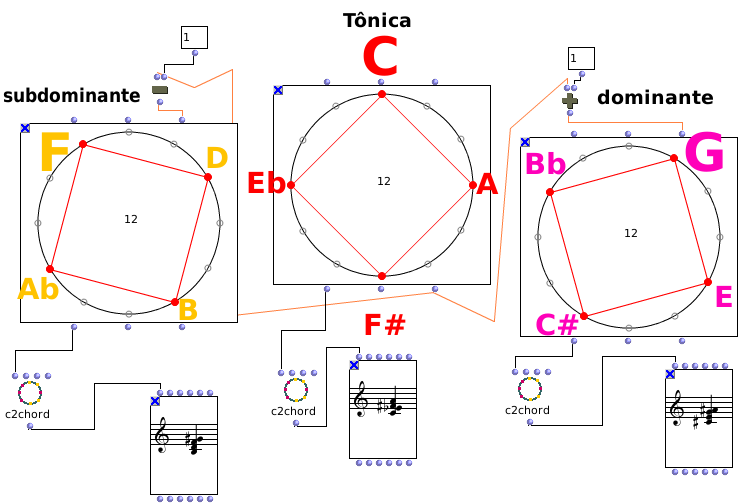
\includegraphics[scale=0.6]{axis/axisOM.png}
	\end{center}
	\legend{Fonte: autor }
\end{figure}


Lendvai chama de \textit{"polo e contrapolo"}\ a relação entre os trítonos nas duas extremidades (que chama de "eixo primário") e observa que o eixo perpendicular (ou "eixo secundário") possui também sua relação de \textit{"polo e contrapolo"}\ entre o que seriam a relativa e a mediante de uma tônica pelo ciclo de quintas. 

A relação entre este \textit{"\textbf{sistema de eixos}"} portanto pode ser a de analogia ao movimento de passo \textit{"$subdominante \leftrightarrow tônica \leftrightarrow dominante$"}\ onde movíamos por passos de 30 graus pelo ciclo de quintas original.  

A diferença é que neste caso a relação mais importante entre as notas do eixo não seria exatamente por um critério baseado na busca de notas comuns de acordes para servirem de pivôs para resoluções tonais ou da busca por notas sensíveis para a solução de dissonâncias por grau conjunto mas uma questão de \textbf{"\textbf{parentesco rotacional}"} das sonoridades dos intervalos que giram de 90 em 90 graus dividindo simetricamente o total cromático numa soma de quatro intervalos de três semitons.

As três transposições possíveis dos eixos de quatro notas tornam a transformação de \textit{"transposição do sistema de eixos"} \textbf{\textbf{\underline{geometricamente}}} similar ao movimento \textit{"$subdominante \leftrightarrow tônica \leftrightarrow dominante$"}\ mas nem sempre pelos mesmos critérios de uma harmonia tonal funcional, apesar de obviamente, poder servir-se deste como estratégia de construção de ambiguidades politonais.

\begin{figure}[!h]
	\caption{\label{fig_grafico}Sistema de Eixos - Rotacão entre primário e secundário}
	\begin{center}
	    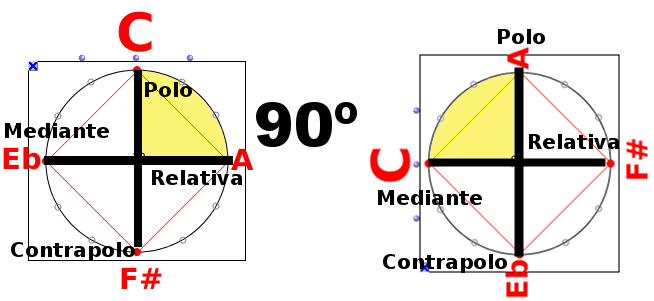
\includegraphics[scale=0.6]{axis/PoloContrapolo.png}
	\end{center}
	\legend{Fonte: autor }
\end{figure}


Lendvai toma este conceito de "polo e contrapolo" como \textit{\textbf{"uma das estratégias estruturais mais fundamentais na música de Béla Bartók"}}\cite[ p.04]{lendvai1971bela} e cita alguns exemplos que confirmam que este tipo de modulação era recorrente.
\pagebreak 
 
Na \textit{"Sonata para dois pianos e Percussão"} o motivo inicial é transposto três vezes com duas vozes em sua relação de trítono \textit{"polo e contrapolo"} e nestas três entradas consecutivas deste motivo é apresentando com as três transposições possíveis do \textit{"sistema de eixos"}, numa relação que pode ser observada como esta analogia com o pêndulo \textit{"subdominante<-tônica>dominante"}: inicia com a relação motívica destacando a relação $C \leftrightarrow F\#$ (compassos 2-5) em seguida (compasso 8) entra o eixo de $G \leftrightarrow Db$ (como se G surgisse de uma relação dominante com C e Db numa simultânea relação dominante com F\#) e nos compassos 12-17 a entrada do jogo entre as transposições $D \leftrightarrow Ab$ como se agora introduzisse a "dominante da dominante"($G \leftrightarrow D$ e $Db \leftrightarrow Ab$) ao mesmo tempo que move-se assim para o último dos três eixos.

\begin{figure}[!h]
	\caption{\label{fig_grafico}O plano melódico do motivo inicial de \textit{"Sonata para dois pianos e Percussão"}  parece ser o de fechar o total cromático com a transposição paralela da melodia nos dois pólos }
	\begin{center}
	    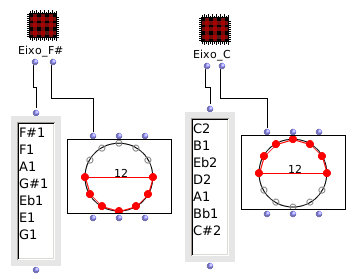
\includegraphics[scale=0.7]{axis/sonata2P_OM.png}
	\end{center}
	\legend{Fonte: autor }
\end{figure}


Podemos observar (Figura 3) que já dentro do motivo inicial temos uma estratégia de entrada de uma coleção de 7 notas a partir de um polo e mais 7 a partir do seu contrapolo em sua voz de resposta - as duas vozes juntas dividem o total cromático em dois, tendo como notas comuns as notas do eixo secundário (a mediante e a relativa - no caso de F\# e C por exemplo, as notas comuns são A e Eb ).

É possível também inferir que a melodia sugere um giro em torno de um eixo que prolonga a expectativa do passo cromático $F\# \rightarrow G$ (e assim por diante em suas transposições). O contorno possui uma simetria no núcleo interno de intervalos com um segmento onde há um salto por quinta invertida no meio de duas células de passo cromático que estão distantes do inicio e do fim da melodia por um salto de 3 semitons (Figura 4). 

Esta estratégia composicional com simetrias internas\footnote{C.f. "Eixo de Inversão"\cite[ p.121]{straus2004}} recorrentes em Bartók por rotações de "células intervalares"\cite[ p.128]{susanni_antokoletz2012music} serão comentadas mais adiante em mais detalhes. 

Lembremos também que as transposições em 3 semitons sugerem esta equivalência de sonoridade das transposições pelo mesmo sistema de eixos usado nas transposições da melodia completa e que o salto em quinta invertida no meio do segmento remete ao ciclo de dominantes tradicionalmente usado para modulações tonais.


\begin{figure}[!h]
	\caption{\label{fig_grafico}Possível estratégia composicional em nível melódico do motivo inicial de \textit{"Sonata para dois pianos e Percussão"}}
	\begin{center}
	    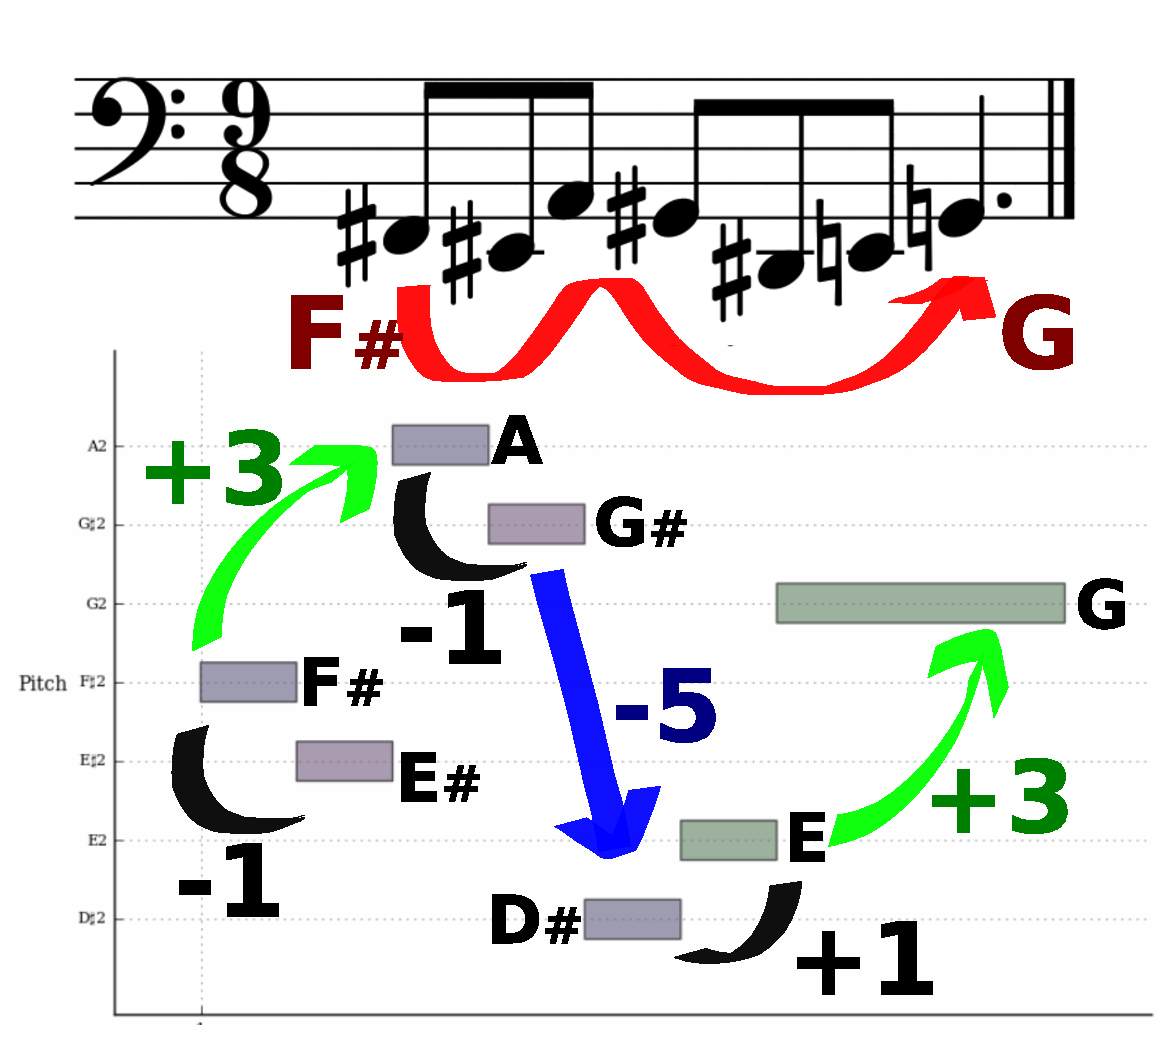
\includegraphics[scale=0.4]{axis/temasonata2P.pdf}
	\end{center}
	\legend{Fonte: autor }
\end{figure}

\citeonline[ p.4]{lendvai1971bela} também lembra situações onde a estratégia de rotação dos polos do sistema de eixos é a conexão entre os movimentos de formas completas, como na opera \textit{"Castelo de Barba Azul"} ($F\# \leftrightarrow  C \leftrightarrow F\#$) e na \textit{"Music for Strings, Percussion and Celesta" } (que altera cada movimento entre os pólos e contrapólos dos eixos primário $F\# \leftrightarrow  C \leftrightarrow F\#$ e secundário $A\# \leftrightarrow  Eb \leftrightarrow A\#$).
\pagebreak


\subsection{A elaboração de uma sonoridade mista maior-menor}

\citeonline[ p.08]{lendvai1971bela} elabora sobre a assimilação do "sistema de eixos"\ na música ocidental como uma evolução natural da harmonia funcional: 

a) O ciclo de dominantes inicia como um sistema de eixos de cadência onde as regiões vizinhas aparecem apenas como função dominante e subdominante sem modulação para outras tonalidades. 

\begin{figure}[!h]
	\caption{\label{fig_grafico}Primeiro estágio: cadencial}
	\begin{center}
	    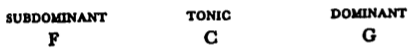
\includegraphics[scale=0.6]{axis/estagio01.png}
	\end{center}
	\legend{Fonte: autor }
\end{figure}


b) O próximo passo é a introdução do eixo da tonalidade relativa (90 graus à esquerda do ponto da tonalidade). A modulação de tonalidade é induzida pela similaridade entre duas regiões diatônicas maiores e menores. Exemplo: Lá menor como relativa de Dó maior e vice-versa.

\begin{figure}[!h]
	\caption{\label{fig_grafico}Segundo estágio: modulação pela relativa}
	\begin{center}
	    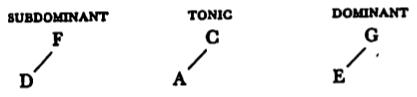
\includegraphics[scale=0.6]{axis/estagio02.png}
	\end{center}
	\legend{Fonte: autor }
\end{figure}


c) No estágio mais avançado do romantismo é introduzido o jogo de ambiguidade entre a tonalidade maior e menor de um mesmo polo permitindo que haja a estratégia de modulação pelo sistema de eixos tanto para 90 graus a esquerda (Ex: Lá menor e Dó maior) quanto 90 graus a direita (Ex: Dó menor e Mi bemol maior ).

\begin{figure}[!h]
	\caption{\label{fig_grafico}Terceiro estágio: modulação pela relativa com ambiguidade maior-menor em um dos polos }
	\begin{center}
	    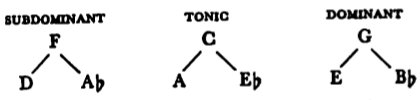
\includegraphics[scale=0.6]{axis/estagio03.png}
	\end{center}
	\legend{Fonte: autor }
\end{figure}


d) Finalmente no último estágio onde e introduzida a politonalidade temos a assimilação da nota que está a 180 graus do polo (relação polo e contrapolo) pela sonoridade almejada de um modo misto "maior-menor"\ e quaisquer um dos pontos, desta maneira um giro completo como $ Dó\ maior-menor \leftrightarrow Lá\ maior-menor \leftrightarrow Fá\ sustenido\ maior -menor \leftrightarrow Mi\ bemol maior-menor \leftrightarrow  Dó maior-menor $ introduz a vertigem de uma sensação de há uma teia de tonalidades simultâneas operando as expectativas de relações entre diferentes eixos.

\begin{figure}[!h]
	\caption{\label{fig_grafico}Quarto estágio: simultaneidade do modos maior-menor permite o jogo de modulações por todos os polos do eixo }
	\begin{center}
	    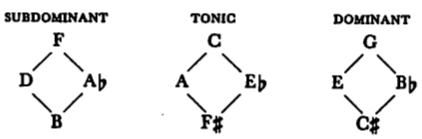
\includegraphics[scale=0.6]{axis/estagio04.png}
	\end{center}
	\legend{Fonte: autor }
\end{figure}



\subsection{Especificidades da coleção acústica (overtone)}

C1, C2, G2, C3, E3, G3, Bb3, C4, D4, E4, F\# 4, G4, A4, Bb4, B4, C5

Uso de overtones com função dominante


Polymode  Lydian-Mixolydian
\cite{suchoff2004bartok}

reflexo de imitação - mikro 29

A peça de número 29, chamada de Reflexo de Imitação divide um aspecto
comum a todas as peças iniciais: a composição baseada em pentacordes associados a um
dedilhado que utiliza os cinco dedos de cada mão. Dessa forma, temos na mão direita o
pentacorde diatônico E- F\# -G\# -A-B e na mão esquerda, outro pentacorde diatônico, o A-B-C-
D-E. Ambos pertencem a mesma classe de conjuntos 5-27 (02357) e se relacionam por
transposição e inversão (T 8 I). A textura
polifônica
e a imitação das vozes em movimento
Reflexo
em Imitação
Béla Bartók
contrário evidenciam essa relação.
( rodrgo-coleção acústica - "compressão intervalar")


comparação entre mkro 29 e 141 ... uso de terminologias de forte
\cite[p. 126]{tymoczko2011geometry}














\subsection{Expectativas de grau sensível}

Substituição da cadência G7 -> C maior pela possibilidade G7->F\# maior-menor (desenhar as setas)

\subsection{Tensões contrapostas de subdominante e dominante}
.

.
.
.


\subsection{Dualidade entre os princípios de tonalidade e distância}

Tríade aumentada C - E - Ab -> "surgindo" da mudança de função "subdominante-tonica-dominante" por uma rotação dos eixos laterais:
(de G pra E e de F para Ab )

.
\subsection{Geometria da Macro-forma com analogias na Micro-forma}

\subsubsection{Secção Áurea}


\subsubsection{Fibonacci}

\subsection{Críticas ao modelo de Lendvai}

\section{Células de Alturas em Antokoletz}


Elliot Antokoletz fundamenta boa parte de sua argumentação em seu livro \textit{"The music of Béla Bartók: a study of tonality and progression in twentieth-century music."}\cite{antokoletz1984music} em torno da ideia de subdivisão da oitava em um complexo de ciclos intervalares rotacionados. Ele insiste por vários ângulos em destacar algumas propriedades da simetria intervalar nas permutações de algumas sequencias recorrentes nas obras do compositor e teoriza sobre a possibilidade de que houvesse uma estratégia de construções transformacionais motívicas destes grupos de intervalos que chama células X, Y e Z. A nomenclatura de sua preferencia - "célula de alturas"(\textit{"pitch cell"}) - é inspirada nos argumentos sobre transformações de grupos motívicos em composição serial proposto por George \citeonline{perle1981serial}. As definções das células X,Y e Z derivam dos estudos bartokianos de \citeonline{perle1955symmetrical} e Leo \citeonline{treitler1959}.

A definição de célula X é baseada em um tetracorde cromático de semitons em sequencia, o que poderia também lembrar o conjunto de Allen Forte de cardinalidade |4-1| - aquele que tem um sua forma normal a sequencia de classes de altura (0,1,2,3). No entanto é bom lembrar que este conceito de células de altura trabalha com uma medida de "intervalo literal" - estão muitas vezes levando em consideração simetrias intervalares que podem estar ocorrendo entre duas oitavas complementares, portanto não são sonoridades agrupadas independentes de âmbito.

A definição de célula Y deriva de uma sequencia em tons inteiros


c.f. "Pitch Cells"
\cite[p.130]{susanni_antokoletz2012music}


\subsection{Ciclos Intervalares}


\begin{figure}[!h]
	\caption{\label{fig_grafico}Ciclos Intervalares observado por \citeonline{antokoletz1984music} - na vertical temos as sequencias (de baixo para cima as distâncias mais curtas e de baixo pra cima suas inversões mais longas). Na horizontal temos em cada coluna da tabela os grupos de transposições possíveis: }
	\begin{center}
	    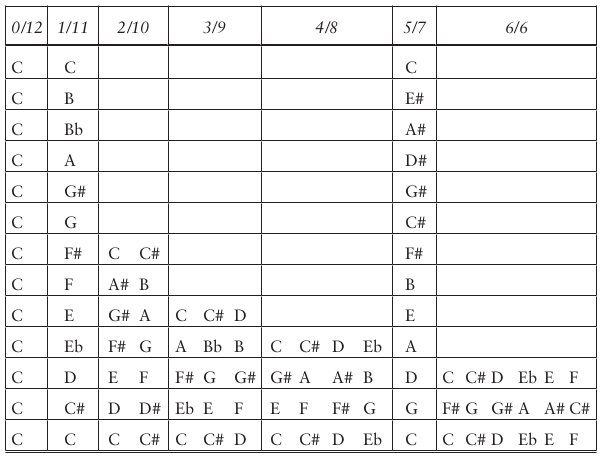
\includegraphics[scale=0.6]{antokoletz/ciclos_intervalares_table2012.png}
	\end{center}
	\legend{Fonte: \cite{susanni_antokoletz2012music} }
\end{figure}



modelo 1:2 , 1:3, 1:5 de Lendvai - pg.51


\section{Modalismo e estratégias rotacionais}

A construção de estratégias composicionais que destacam identidades de escalas modais é traço fundamental para entendimento de repertórios que buscavam hibridizar melodias populares com arranjos e harmonizações da música artística ocidental nas primeiras décadas do século XX. 

Apesar da música de Bartók ser frequentemente associada a um apelo folclorista, devido a suas pesquisas na música camponesa do leste europeu que sempre influenciaram seu trabalho, é importante destacar que Bartók sempre o fez aproximando as melodias de uma linguagem moderna e proto-serialista, ainda mais depois de exilado nos Estados Unidos e obviamente tocado pela catástrofe que derivou dos nacionalismos que racharam a Europa nas duas guerra mundiais que presenciou.\footnote{Um exemplo simples e curioso é a modificação sarcástica do tema do Hino Austríaco demonstrada por \citeonline[ p.2934]{suchoff1971guide}. }

Danielle \citeonline{fosler2007music} aponta ainda de maneira interessante em seu livro \textit{"Music divided: Bartók's legacy in cold war culture"}\ algumas evidências de que por fatores como a morte de Bartók logo após a segunda guerra mundial (1945) e a singularidade de representar a figura de um exilado que trabalhou no limite entre a linguagem de pesquisa da tradição de sua terra natal e invenção contemporânea universal, Bartók influenciou tanto músicos de vanguarda do serialismo quanto revisionistas da música artística inspirada em motivos populares.

É essencial portanto, apontar aqui algumas maneiras pelas quais motivos de característica mais folclórica foram usados em sua linguagem de maneira a criarem texturas que assimilam transformações pós-tonais criando sonoridades polimodais, cromáticas e de um serialismo de forte apelo motívico.

\citeonline{susanni_antokoletz2012music} demonstram de maneira bastante pedagógica algumas técnicas de rotação intervalar, transposição, união e mistura de coleções modais por inserção de notas pivô e a transformação orgânica de motivos modais ou pentatônicos em novas sonoridades híbridas não-diatônicas, cíclicas e de uma ambiguidade maior-menor, presente nesta linguagem. Veremos a seguir.

\subsection{Rotação Pentatônica}
 
Da mesma maneira que tradicionalmente pensamos a rotação da coleção diatônica nas notas brancas do piano para memorizarmos os modos gregos, como por exemplo chamar as melodias iniciadas em Ré de "Modo Dórico" e dela poder entender sua série intervalar fixa de \textit{"0,2,3,5,7,9,10,12..."} que pode ser transposto; podemos também aplicar a ideia de rotação nas "notas pretas do piano" e considerar algumas propriedades das sequencias de intervalos gerados para a sequencia intervalar \textit{"0,2,5,7,9,12..."}.

\citeonline[ p.83]{susanni_antokoletz2012music} trabalham esta ideia comum no repertório pós-tonal de fazer a rotação da pentatônica criando uma estratégia para gerar ambiguidade em relação aos modos gregos, já que as pentatônicas não possuem os semitons que as caracterizam. Podemos então jogar com as notas faltantes como pivôs de uma transformação entre diferentes modos ou de uma simultaneidade que Bartók chamou "polimodalismo cromático" e que falaremos mais adiante. 

Se considerarmos a normalização da sequencia tradicional das notas pretas como a transposição para os intervalos a partir de Dó ( $C \rightarrow  D \rightarrow F \rightarrow G \rightarrow A \rightarrow C $ ) , teremos a sequencia de intervalos de semitom ( $C \rightarrow 2 \rightarrow  3 \rightarrow 2 \rightarrow 2  \rightarrow 3 \rightarrow C $ ). Iniciando a partir de Ré (chamemos aqui de \textbf{"rotação 2"}) teremos a rotação e intervalos ($D \rightarrow F \rightarrow G \rightarrow A \rightarrow C \rightarrow D $ ) equivalente a ( $  D \rightarrow 3 \rightarrow  2 \rightarrow 2 \rightarrow 3  \rightarrow 2 \rightarrow D $ ) e assim por diante.\footnote{Interessante notar aqui que a pentatônica a partir de Sol gera uma sequencia de intervalos que pode ser particionada simetricamente. Veremos na Sessão mais adiante estratégias de uso das simetrias.}

Pensemos também que a partir desta configuração de intervalos podemos normalizar todas as sequencias em uma mesma nota raiz de transposição. Por exemplo, a partir de Dó a sequencia intervalar demostrada no parágrafo anterior como a \textbf{"rotação 2"} é transposta como ($C \rightarrow Eb \rightarrow F \rightarrow G \rightarrow Bb \rightarrow C $ ).

É a partir disso que \citeonline[ p.84]{susanni_antokoletz2012music} que estas rotações da pentatônica e suas transposições servem como uma maneira de construir transformações entre diferentes modos usando como pivô uma ou mais rotações ou transposições de um motivo pentatônico. 

Por exemplo, uma estratégia de ambiguidade entre modo Lídio e Mixolídio:
\linebreak
Pentatônica: $ C - D \rightarrow [ ?? ] - E - G - A \rightarrow [ ?? ] - (...) $  \linebreak
******Lídio: $ C - D \rightarrow [ $F\#$ ] - E - G - A \rightarrow [ B ] - (...) $  \linebreak
**Mixolídio: $ C - D \rightarrow [ F ] - E - G - A \rightarrow [ Bb ] - (...) $  \linebreak

A inserção de jogos de tensão com a célula [ B - F\# - F - Bb ], mostra-se portanto uma estratégia possível para as transições deste polimodo.

%serie acústica:
%C1, C2, G2, C3, E3, G3, Bb3, C4, D4, E4, F\# 4, G4, A4, Bb4, B4, C5

%mikrokosmos 29

%modelo diatoônico de lendvai

%alpha cord invertido




 
%%%%%%% encontrar exemplo de pentatonica e modo lidio-mixolodio no bartok

  



\section{Simetria Inversiva}

Edward \citeonline{pearsall2004symmetry} observa que já no motivo inicial, que serve de "célula germinativa"\ para outras transformações na peça a construção simétrica esta presente tanto na construção do eixo [1,5,1] (Figura) nos intervalos melódicos como na construção de uma citação simétrica de uma escala completa de oito tons, que seria cortada ao meio por um intervalo ausente de C\# (Figura).

\begin{figure}[!h]
	\caption{\label{fig_grafico}Exposição das primeiras citações do intervalo 151 e sua dissolução por rotações e inserção de novos intervalos. Código do script gerador no apêndice.}
	\begin{center}
	    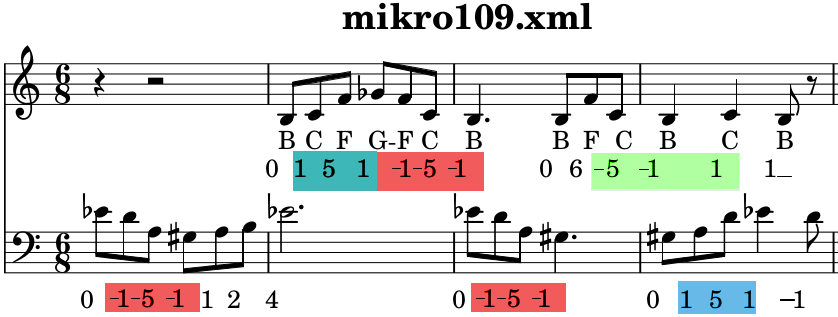
\includegraphics[scale=0.5]{estudosM21/contornoM109.png}
	\end{center}
	\legend{Fonte: autor }
\end{figure}





\subsection{Simetria Literal}


George Perle, apesar de também ter sido um entusiasta dos apontamentos motívicos em Bartók, alerta para o problema da definição de uma forma de macroestrutura não ser suficientemente determinada por estes achados de estratégias internas de construções simétricas:

\begin{citacao}
Impressive as these procedures are, it must be observed that Bartk's symmetrical formations 
are only an incidental aspect of his total compositional means. Even in those few works where they perform a significant structural role they do not ultimately define the context, which is determined
instead by a curious amalgam of various elements..
Can symmetrical formations generate a total musical structure, as triadic relations have done traditionally? The implications of Bartók's work in this, as in other aspects, remain problematical.
\end{citacao}

Como proposta para entender coerências macroestruturais para as simetrias na música de Bartók, Joseph \citeonline{bernard1986space} propõe a observação do que chama \textit{"simetria literal"}\ destacando a estratégia composicional por uma conjunção de simetrias intervalares que podem espalhar-se por todo âmbito de oitavas usado numa composição.  

Funciona como um  agregado sonoro que cria uma expectativa de equidistância de uma nota central em um grupo de intervalos - seja uma sequencia de notas em forma melódica ou um cluster vertical. 

Por exemplo: { Db3, C4, B4} possuem entre si as distancias [-11 ,0 ,11 ] se considerarmos o C4 como um centro, mas se usarmos o mesmo agrupamento dentro de uma única oitava {Db4-C4-B4} teremos as distâncias [ -1, 0, 11] onde apesar de podermos considerar os intervalos [1,11] inversivamente equivalentes por inversão\footnote{Com base nas "teorias de grupos das classes de altura".} não teremos esta sonoridade de equidistância dentro de um eixo de 22 semitons, que funcionaria como um eixo estratégico na composição dos jogos simétricos de um peça que use a simetria literal. 

Bernard localiza no ensaio "Problems of New Music" do proprio Bartók com o nome de \textit{\textbf{"simetria em espelho"}}.


figuras da  \cite[p. 187]{bernard1986space}

\citeonline[p. 189]{bernard1986space} localiza um exemplo aplicado no Concerto n.2 para piano e Orquestra de Bartok uma estrutura de construção de simetrias por alternancia de tons e semitons ao longo de um registro que vai de F4 descendo a C0 nos 5 primeiros compassos e de C5 a Eb0 nos compassos de 6 a 8.

A peça Mikrokosmos n.141 já sugere o procedimento no próprio título "Sujeito e Reflexão".

The piece consists of a series of short sections, each of which is symmetrical about a single
pitch or a pair of pitches one or more octaves apart.\cite[p. 187]{bernard1986space}

Closely related to parallel and mirror symmetry respectively are replica-
tion and inversion. The only difference is that replication and inversion are
better suited to describing order of events, in which a given configuration
may be said to give rise to another.\cite[p. 190]{bernard1986space}


simetria por eixo em sonata para 2 pianos \cite[p. 195-198]{bernard1986space}



"simetria inversiva"
"combinação transposicional"
\cite{cohn1988inversional}

One senses in Bart6k's total output an all-encompassing
system of pitch-relations. The present study is intended to demonstrate that
Bart6k's music is indeed based on such a system.... Pitch relations
in Bart6k's music are primarily
based on the principle of equal subdi-
visions of the octave into the total complex of interval cycles. The fun-
this equal-division
damental concept underlying
system is that of sym-
metry.


Bartók clearly favored the fifteen inversionally
symmetric tetrachord-classes, in particular those thirteen which
are capable of being realized as symmetric four note pitch-sets.
(The two exceptions are 4-6 [0127] and 4-24 [0248].) The thir-
teen include 4-1 [0123], 4-21 [0246], and 4-9 [0167], which figure
prominently in the writings of Perle and Antokoletz, where
they are called X, Y, and Z cells; 4-17 [0347], Lendvai's
"gamma" chord;11 and 4-3 [0134] and 4-10 [0235], the half-
octatonic tetrachords discussed by Berry.




Example 2a brackets two versions of the four-note motive found in
bb. 1-3 of Bartók's Mikrokosmos, Vol. IV, no. 94, 'From the Island of
Bali'. The first of these motives outlines a descent with the interval
succession 1 / 5/1. This motive - which itself represents a symmetrical
structure in pitch space - forms the basis for a series of motivic trans-
formations that propel the piece forward. In b. 2, the motive turns
upside down, increasing the range of the composition and adding
several new pitches. Taken together, the two pitch collections in bb. 1
and 2 form a one-octave octatonic scale. This symmetrical scale, shown
in Ex. 2b, projects a 1/2 interval series above and below C\#, the axis of
inversion.4 As the piece continues, the motive begins to degenerate
through truncation and reordering, as shown in Ex. 2c. The degenera-
tion of the motive also has the effect of dissolving the symmetry of the
pitch collection. Symmetry is restored in b. 12 where the complete
motive and its inversion return. The piece ends with the symmetrical
collection shown in Ex. 2d. This collection is also drawn from the
octatonic scale, but occupies a broader region in pitch space. Here, the
notes of the opening 1 / 5 / 1 gesture are presented as chords, helping to
highlight the intervallic symmetry of the collection.

(bartokcrumbmikro.pdf )


\section{Coleções referenciais ordenadas por conjuntos de classes de altura}

O uso sistemático de uma teoria unificada para a classificação de classes de altura em conjuntos relacionados por transposição, inversão, complemento, simetria e outras possíveis observações de propriedades específicas de agrupamentos intervalares tem a sua disposição a construção de alguns consensos que giram sobretudo em torno de uma área da musicologia de origem norte-americana\footnote{Sobre a influência da \textit{"Teoria dos Conjuntos de Classes de Altura"} norte-americana na musicologia européia ver \citeonline{aroundset2013}.} que tem se estruturado desde fortalecimento acadêmico do serialismo na segunda metade do século XX. Geralmente é referida como \textit{"Pitch Class Set Theory"}, e normalmente traduzida para português pelo termo \textit{"Teoria dos Conjuntos de Classes de Altura"}\cite{straus2004}.

\begin{citacao}
Foi, obviamente, Allen Forte quem foi o pioneiro das análises com a taxonomia dos \textbf{conjuntos de classes de alturas} aplicadas em conceitos da matemática, primeiro surgindo em tipos de Milton Babbit (a teoria conceitual), e em seguida com a inclusão e abstração de relações (como as relações de similaridade) construídas para uso analítico. A \textbf{"teoria de conjuntos"}\ de Forte (...) tem tido suas próprias ramificações e influência. Em particular, as próprias análises de Forte de peças individuais tem levado muitos outros a fazerem de maneira parecida, e a ideia inicial de Forte das relações de similaridade ( diferentes das relações de equivalência) sobre os grupos de classes de alturas tem visto florescer uma indústria teórica em torno disto, depois que os artigos seminais de Morris, Rahn  Lewin apareceram em 1980. \cite[ p. 130]{rahn2004swerve}\footnote{
It was, of course, Allen Forte who in the USA pioneered the analytical with a taxonomy of pc-set application of concepts from mathematics, first arose also in serial Babbittian types (the concept theory), and following as some inclusion and with relations abstract up (such similarity relations) meant for analytical use. Forte's "set theory"\  (...) has had its own ramifications and influence. In particular, Forte's own analyses of individual pieces of music have led many others to do likewise, and Forte's initial idea of similarity relations (as distinct from equivalence relations) among pitch-class sets has seen a flourishing theoretical industry grow around it, after seminal articles by Morris, Rahn, and Lewin appeared in 1980. \cite[ p. 130, grifo nossos]{rahn2004swerve}}
\end{citacao}

Para uma introdução resumida da terminologia da T.C.C.A. sugerimos a consulta do Apêndice do presente trabalho e dos patches de OpenMusic disponibilizados para sua demonstração. Para uma introdução mais aprofundada que serviu como referência aqui sugerimos a tradução brasileira do livro de \citeonline{straus2004} e os trabalhos originais de \citeonline{forte1973structure} e \citeonline{rahn1980basic}.

Observamos a seguir um exemplo de análise de inspiração na T.C.C.A. que utiliza como base discussões sobre a coleção referencial octatônica - grupos de oito intervalos separados entre duas oitavas por uma sequencia não-diatônica que intercala tom e semitom, gerando propriedades curiosas e de bastante uso na música de Bartók e no repertório pós-tonal em geral.




\subsection{Octatonismo e suas partições}

Richard \citeonline{cohn1991bartok} propõe em seu artigo \textit{"Bartók's octatonic strategies: a motivic approach"}\ uma abordagem que utiliza a nomenclatura dos conjuntos de classes de altura propostas por Allen \citeonline{forte1973structure} na tentativa de construir um discurso sobre as coleções de sonoridades em Bartók que articule com uma continuidade das tradições analíticas.

Considera importante sistematizar aspectos transpositivos, inversivos e relações intervalares com lastro na harmonia funcional. Para isso traça uma estratégia que parte do mapeamento de permutações da coleção octatônica separando desta também derivações de díades e tétrades pelo que chama de "grau de fertilidade"\cite[ p.268]{cohn1991bartok} - a capacidade do segmento em relacionar-se por transposição com outros grupos de mesma cardinalidade (mesmo número de elementos).

Ao separar os grupos em pares relacionados por transposição, Cohn almeja encontrar um sistema de classificação de intervalos também por sua funcionalidade em parte da expectativa politonal que também rege estas obras:

\begin{citacao}
Pairs of notes are classified either by interval-class or by dyad-class in this study.
The two classifications are identical, so their distinction is a matter of orientation. As
with interval-classes, names of dyad-classes correspond to the smallest interval, measured in half-steps, available between their constituent pitch-classes. Thus dyad-class I includes pairs of pitches separated by half-step, major seventh, and their enharmonic equivalents and compounds; dyad-class 2 includes whole-steps, minor sevenths, and their enharmonic equivalents and compounds, and so forth up to
dyad-class 6, the tritone. Although theorists use interval-class more frequently, the
concept of dyad-class allows for a more natural comparison to larger sets.
\cite[ p.265-266]{cohn1991bartok}
\end{citacao}





\section{Harmonização dos Modos Folclóricos}


A harmonização  bartokiana em muitos casos é desamarrada das cadências tonais pela intenção de destacar a sensação modal ou pentatônica das melodias. Esta foi também uma estratégia para criar harmonizações onde as tríades maior e menor são usadas de modo ambíguo, simultâneo e que facilitam o uso do total cromático. Também ao evitar a sensível surge a preferência do uso de intervalo de sétima menor como uma sonoridade sem expectativa de resolução de tonalidade que torna na música de Bartók este intervalo um traço "tão importante quanto as observação das terças e quintas na harmonia funcional tonal"\cite[p. 28]{antokoletz1984music}.

Nas palavras do próprio Bartok:

\begin{citacao}
"Quanto mais simples a melodia mais complexa e estranha pode ser a harmonização e acompanhamento que vai bem com esta(...) Estas melodias primitivas, de alguma maneira, não mostram traço de junção estereotipada das tríades(...) Isto nos permite trazer a melodia mais claramente ao construir harmonias de espectro mais amplo variando ao longo de diferentes polarizações"
\cite[p. 342]{bartok1993bela}
\end{citacao}


Bartók concluded:
each tone is used as an independent degree. Therefore these scales ought to be regarded as a segment-a kind of
pentachord-of a twelve-hemitone [sic] scale; but, of course, with a fixed tonality because of their ever
recurring, never changing final note.10

In the third 'Harvard Lecture', on 'Chromaticism', presented in February 1943,
Bart6k talked at length about these structural chromatic melodies from Algeria and
Dalmatia, relating his comments to the 'new chromatic' melodies in his compositions:

As to the general characteristics, exactly the same can be said about my melodies as what I said already
concerning the chromatic folk melodies. That is, the single tones of these melodies are independent tones
having no interrelation between each other. There is in each specimen, however, a decidedly fixed
fundamental tone to which the other tones resolve in the end. The main difference between the chromatic folk
melodies and my own chromatic melodies is to be found in their range. They consist exclusively of five, six, or
at most seven half-tones, which corresponds to a range of about a fourth. My own melodies generally have at
least eight half-tones and cover, in some cases, the distance of an octave or more. 1
\cite[ p.6]{gillies1983bartok}










acordes usados de maneira “livre” para harmonizar notas melódicas que não pertencem a estes

na bagatela numero 4 o tecido harmônico é determinado basicamente por um sistema de ambiguidade maior-menor 

evitando o leading-tone (sensível) – exemplo D menor (eólio) . Evita acorde de sétima maior. 
A tríade construída sobre o quinto grau não faz o mesmo papel que na musica tonal tradicional.

A função do acorde de sétima menor faz o papel modal , evitando a ideia de resolução eminente de uma tonalidade maior ou menor.

O acorde de sétima menor possui uma propriedade de simetria interna dos intervalos. Metade do acorde espelha outra metade. Este equilíbrio contribui para uma sensação de imobilidade aparente. Neutralidade Cinética.



Um exemplo citado no livro de  \citeonline{suchoff2004bartok} dedicado exclusivamente aos mikrokosmos é da primeira canção folk tratada na coleção.

A Melodia pentatônica é também uma estratégia para introduzir uma célula de uma coleção octatônica.

Aplicamos aqui os algoritmos de análise de harmonia funcional da biblioteca music21.

\subsection{Limites e ideias a partir de analise tonal funcional}

comparação recente com algoritmo de key probing
\cite{cooper1998unfolding}


usar analise comentario mikro 100 e 101 do paper 25bartokshenker limits
\cite[ p.179]{brown1997iv}

mikro101
\cite[ p.113]{straus2004}

\subsection{Acompanhamento e textura}

\cite{starr1985melody}


\subsection{Centricidade por Equilíbrio Inversivo}
Às vezes a idéia do equilíbrio inversivo em torno de um eixo pode afetar mais do que
apenas um único conjunto de classe de notas ou grupo de conjuntos. Ela pode expandir-se
para abranger todas as doze classes de notas. Nesse caso, cada classe de notas mapeia-se
em outra (ou nela mesma) em torno de algum eixo. A Bagatela, Op. 6, No 2, de Bartók,
começa com notas Láb e Sib repetidas na mão direita (ver o Exemplo 4–14).

Uma melodia começa no compasso 3 em Sin, um semitom acima da figura repetida, e
então continua com Sol, um semitom abaixo da figura repetida. Depois vem Dó e Solb
(dois semitons acima e abaixo), Réb e Fá (três semitons acima e abaixo), Ré e Fáb (quatro
semitons acima e abaixo), e finalmente Mib, uma classe de notas que está cinco semitons
tanto acima quanto abaixo. A única classe de notas que não foi ouvida é Lá, que está
justamente no meio da figura repetida, um tipo de centro silencioso em torno do qual tudo
se equilibra (ver a Figura 4–8).
\cite[ p.121]{straus2004}


%
%
%
%%%%%%%%%%%%%%%%%%%%%%%%%%%%%%%%%%%%%%%%%

\part{Formalizações Computacionais}

\section{Analise de Corpus}

\subsection{Formatos de entrada}

\section{Music21}

É uma biblioteca projetada para trabalhar com manipulação e análise de \textit{corpus} de arquivos partituráveis\footnote{\url{http://web.mit.edu/music21/doc/moduleReference/moduleCorpus.html} Acesso em 10 de julho de 2014.}. Prepara a conversão entre diversos arquivos de dados musicais (MIDIs, humdrum, lilypond, abc)\footnote{\url{http://web.mit.edu/music21/doc/moduleReference/moduleConverter.html} Acesso em 10 de julho de 2014.}, mas nativamente trabalha com uma estrutura de dados baseada em Music XML.

Music21 tem uma abordagem voltada para uma "musicologia assistida por computador"\ e já tem incorporada em suas classes algumas ferramentas comuns a esta prática como: numeração de grau funcional de acorde\footnote{\url{http://web.mit.edu/music21/doc/moduleReference/moduleRoman.html} Acesso em 10 de julho de 2014.}, numeração de classes de altura usando a classificação de Allen Forte\footnote{\url{http://web.mit.edu/music21/doc/moduleReference/moduleChord.html?\#music21.chord.Chord.forteClassNumber} Acesso em 10 de julho de 2014.} e a implementação dos algoritmos de detecção de tonalidade\footnote{\url{http://web.mit.edu/music21/doc/moduleReference/moduleAnalysisDiscrete.html} Acesso em 10 de julho de 2014.} elaborado por \citeonline{krumhansl1990cognitive} e aperfeiçoado por \citeonline{temperley2001cognition}, descritos nesta pesquisa.\footnote{\autoref{perfiltonal}}

\subsection{Stream}


\subsection{Notas, Acordes e nomenclaturas}


\subsection{Prolongamentos e inferência de tonalidade}

\subsection{Key Profiles}

\subsection{Escalas e Modalismo}

\subsection{Contorno melodico}

\subsection{Metrica composta}

\subsection{Acento Melodico}

\subsection{Busca e extraçao de padroes}

Com music21 a possibilidade de tornar a segmentação independente do gesto gráfico

\section{OpenMusic}

as vantagens de segmentaçao via mouse. LZ , Inerface de analise e SOAL como exemplos de possivel automacao do procedimento usando LISP ou servidores externos.

\subsection{Visualização das classes de altura}

\subsection{Manipulação de Conjuntos e suas nomenclaturas}

\subsection{"Sieves" de ciclos intervalares}

\subsection{Segmentação Monitorada}


\section{Especialidade da automação versus especialidade do analista}

problema ou utopia da "analise cega"


\chapter{Composição Assistida por Computador}

\section{Cliches generativos partituraveis}



\section{Formatos de saída}

\section{Tecnicas em Music21}

\section{Experimentos em outras linguagens de CAC}

\subsection{Tecnicas em OpenMusic}

\subsection{Problematizações em PureData}

\section{Probabilidade e Combinatória}




%%%%%
%%%%%
%%%%%
%%%%%
\part{Experimentos Generativos}

\chapter{CosmoBagatellas}


\chapter{Lastros e Rumos}


%%%%%
%%%%%
%%%%%
%%%%%



% ----------------------------------------------------------
% ELEMENTOS PÓS-TEXTUAIS
% ----------------------------------------------------------
\postextual
% ----------------------------------------------------------

% ----------------------------------------------------------
% Referências bibliográficas
% ----------------------------------------------------------
%\bibliography{abntex2-modelo-references}
\bibliography{mestrado_glerm}
% ----------------------------------------------------------
% Glossário
% ----------------------------------------------------------
%
% Consulte o manual da classe abntex2 para orientações sobre o glossário.
%
%\glossary

% ----------------------------------------------------------
% Apêndices
% ----------------------------------------------------------

% ---
% Inicia os apêndices
% ---
\begin{apendicesenv}

% Imprime uma página indicando o início dos apêndices
\partapendices

\chapter{Fórmulas de agrupamento e transformação dos intervalos}

A teoria de grupos de classes de altura utiliza como base de suas formulações a relação entre os 12 semitons da escala cromática de forma modular: considerando alturas de mesma oitava como sujeitas mesmas propriedades intervalares, podendo argumentar relações independentes de registro. Exemplo: O Dó grave representado no protocolo MIDI pelo valor 24 tem uma relação de equivalência com o Dó agudo de valor 72. A fórmula é simples: ambos quando divididos por 12 apresentam resto 0. A nota Ré, por exemplo, sempre apresentaria o resto 2, e assim por diante. Dizemos por tanto que pertencem a uma mesma classe de altura.

Diferente de quando argumentada uma enarmonia funcional\footnote{ver \autoref{solfejo} } (como por exemplo D\# $\to$ Eb ) a teoria de grupos e classes de altura não toma como princípio ideias do tipo "terça maior ou menor", "nota sensível" ou "nota de passagem"\ pois vai partir de uma relação direta entre os aglomerados sonoros, buscando similaridades e equivalências sem estar tão presa as formas de prolongamento normatizadas pelo tonalismo clássico. \cite{lerdahl1989atonal,straus1987problem}

Os intervalos são, sobretudo, distâncias. Nas teorias de classes de alturas essas distâncias podem estar categorizadas como intervalos ordenados - usando número negativos para os intervalos descendentes, ou não-ordenados - considerando intervalos equivalentes independentes de suas direções.\cite[p. 6]{straus2004}

Isso cria imediatamente uma relação interessante de parentesco entre pares em todos intervalos da escala cromática - exceto para o trítono, intervalo de sexta ordem que esta equidistante de 0 e 12 e portanto não possui uma inversão propriamente dita, mas sim tem o papel de cortar ao meio este espelhamento.

\begin{figure}[!h]
	\caption{\label{fig_grafico}Equivalência de intervalos por inversão }
	\begin{center}
	    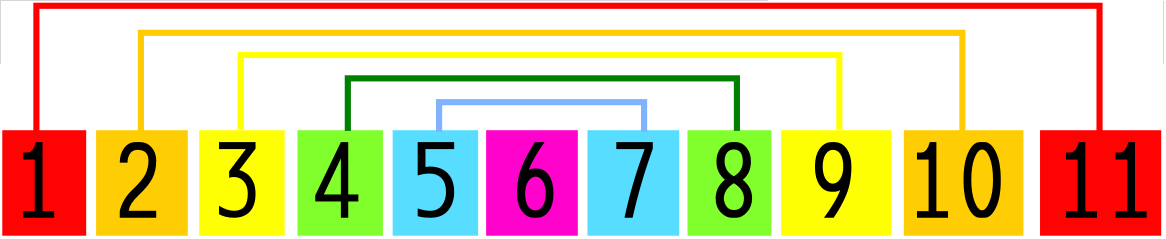
\includegraphics[scale=0.3]{algo/equivalencia_inversa.png}
	\end{center}
	\legend{Fonte: autor }
\end{figure}


\section{Vetor intervalar}

A operação obtenção do vetor intervalar é a primeira das reduções sugeridas para propor uma similaridade entre agrupamentos que seja neutra quanto a inversões e oitavas.

Tomemos um exemplo de uma sequência C-D-E-Bb.



\begin{figure}[!h]
	\caption{\label{fig_grafico}[0,2,4,10] }
	\begin{center}
	    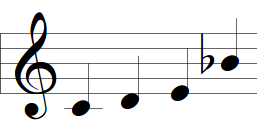
\includegraphics[scale=0.6]{OM_settheory/vetor02410.png}
	\end{center}
	\legend{Fonte: autor }
\end{figure}


Este trecho pode ser reduzido a sequência de alturas [0,2,4,10]

Organizamos seus intervalos fazendo todas as combinações possíveis entre essas distâncias:


$ inversões = \left\{
  \begin{array}{l l}
    2-0 = 2\\
    4-0 = 4\\
    10-0 = 10 \\
     \\
    4-2 = 2\\
    10-2= 8 \\
     \\
    10-4= 6
  \end{array} \right.
$

O vetor de intervalos pode ser reduzido então a uma contagem que coloca no mesmo grupo os intervalos que são inversões dos primeiros cinco intervalos possíveis, já que seus pares após o trítono não são considerados espelhamentos. No exemplo acima temos 10 que é a inversão de 2 e 8 que é a inversão de 4. Nosso vetor fica assim:


\begin{table}[h]
\begin{tabular}{|
>{\columncolor[HTML]{FD6864}}l |
>{\columncolor[HTML]{F8A102}}l |
>{\columncolor[HTML]{F8FF00}}l |
>{\columncolor[HTML]{34FF34}}l |
>{\columncolor[HTML]{00D2CB}}l |
>{\columncolor[HTML]{EE00EE}}l |}
\hline
1 & 2 & 3 & 4 & 5 & 6 \\ \hline
0 & 3 & 0 & 2 & 0 & 1 \\ \hline
\end{tabular}
\end{table}

Pode-se dizer então que a classe de alturas [0,2,4,10] possui o vetor intervalar <0,3,0,2,0,1>.


\section{Forma Normal} 

É comum na prática de uso dos grupos de classes de altura a preparação dos conjuntos em sua forma ordenada e reduzida. Desta maneira podemos mais facilmente reconhecer as equivalências entre os grupos, reconhecer transposições, propriedades.


\begin{figure}[h]
	\caption{\label{fig_grafico}Redução de um segmento do Microkosmos 101 de Bártok para um cluster de 4 alturas. }
	\begin{center}
	    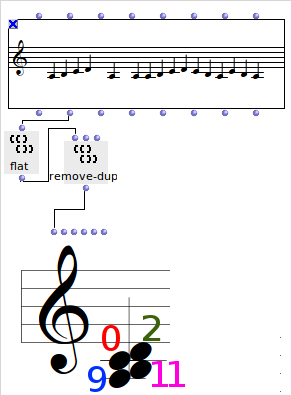
\includegraphics[scale=0.7]{OM_settheory/reducao_acorde.png}
	\end{center}
	\legend{Fonte: autor }
\end{figure}

Para a redução de uma forma normal, partimos do \textit{cluster} sem repetições, colocando todas as alturas dentro da mesma oitava. Os passos seguintes são: 
\textbf{a)} Ordenar de forma ascendente e escolher a sequência que tenha a menor distância da primeira até a última nota.
\textbf{b)} Se houver empate reduzir pela que seja mais compacta à esquerda, comparando o menor intervalo entre a primeira e penúltima e assim por diante.
\textbf{c)} Havendo ainda empate, escolher aquele grupo que tem a menor altura como início. 

\begin{figure}[h]
	\caption{\label{fig_grafico}Forma Normal. }
	\begin{center}
	    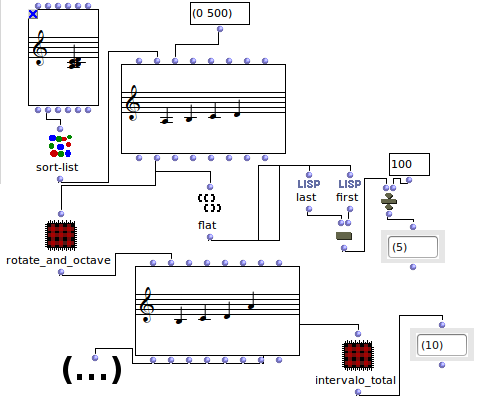
\includegraphics[scale=0.7]{OM_settheory/forma_normal.png}
	\end{center}
	\legend{Fonte: autor }
\end{figure}



\pagebreak
\section{Forma Prima} 

A forma prima é um procedimento para simplificar ainda mais a forma normal, encontrando "a mais normal das normais"\ \cite[p. 47]{straus2004} e reduzindo vetores que possuem os mesmos intervalos ou são inversões e transposições a um vetor primário. Para isso uma forma normal é transposta até que possua o zero em sua primeira posição. Assim é feito também com sua inversão. A forma mais compacta à esquerda será a forma prima. Allen \citeonline{forte1973structure} desenvolveu uma taxonomia a partir das formas primas que tem sido utilizada como forma canônica para representação de grupos de classes de altura.\footnote{A biblioteca \textit{"math"}\ do OpenMusic possui o objeto "p-form"\ para encontrar os agrupamentos de Forte. A tabela original está no livro "The Structure of Atonal Music"\ \cite[p.179-181]{forte1973structure}}. Forte organiza agrupamentos pelo número de elementos seguidos por um número que diz qual ordem dentro do conjunto com aquele mesmo número de elementos. Exemplo: |3-1| é composto das alturas (0,1,2), |3-2|  é o cluster (0,1,3), |4-17|  é composto por (0,3,4,7), e assim por diante.

\begin{figure}[h]
	\caption{\label{fig_grafico}Fórmulas de agrupamento de classes de altura. }
	\begin{center}
	    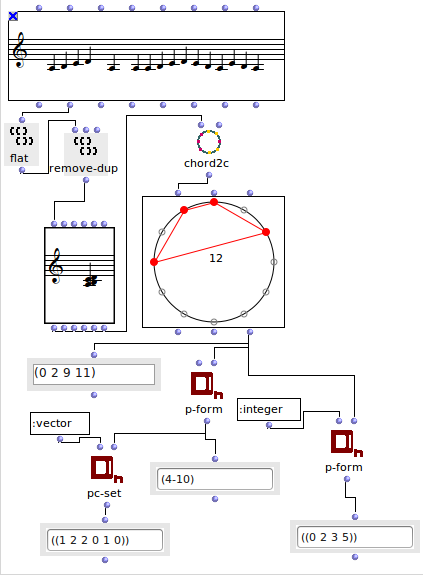
\includegraphics[scale=0.7]{OM_settheory/forma_prima_forte_vector.png}
	\end{center}
	\legend{Fonte: autor }
\end{figure}


\section{Singularidades nos agrupamentos }

Algumas propriedades entre os grupos de classes de alturas são muito interessantes como princípio composicional e, mesmo quando não tão obvias em primeiras audições, ao menos ajudam garantir alguma coerência estrutural conceitual. George Perle argumenta sobre "funções motívicas"\ em grupos de alturas \cite[ p.60-85]{perle1991serial} e observa algumas estratégias de compositores para aproveitar algumas propriedades encontradas em relações internas das series. Perle no entanto mostra-se cético quanto a formalização de nomenclaturas analíticas derivadas da classificação de Allen Forte e sua aplicação em argumentações para análises de composições que tenham sido compostas antes fórmulas tornarem-se ferramentas musicológicas. \cite{perle1990pitch}

Levantaremos aqui algumas destas propriedades conforme o resumo didático proposto por \citeonline{straus2004}, sem ainda estarmos certos de sua efetividade para analises mas interessados na formalização computacional possível destas para processos composicionais.


\subsection{Notas comuns sob transposição}

Tomemos o seguinte exemplo: Dado um grupo em sua forma prima [0,2,5] - ou "4-10"\ na forma prima pela classificação de Allen \citeonline{forte1973structure} - quando transpomos para o intervalo 2 e seu inverso 10, obtemos duas notas iguais para cada um destes grupos.

\begin{figure}[!h]
	\caption{\label{fig_grafico}Notas comuns na transposição. }
	\begin{center}
	    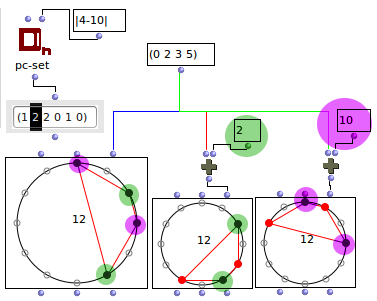
\includegraphics[scale=0.7]{OM_settheory/notas_comuns_2e10.png}
	\end{center}
	\legend{Fonte: autor }
\end{figure}



Isso acontece porque o vetor de intervalos para esta forma é <1,2,2,0,1,0> e podemos observar que há uma fórmula geral que prova que o número de incidências comuns de uma determinada classe de alturas em sua transposição será o número de repetições deste intervalo em seu vetor original. Neste caso por exemplo temos duas incidências do intervalo de classe 2 - portanto as transposições T2 e T10 tem duas notas em comum com T0.

Há uma exceção a esta regra:
 
\begin{figure}[!h]
	\caption{\label{fig_grafico}Notas comuns na transposição com trítono. }
	\begin{center}
	    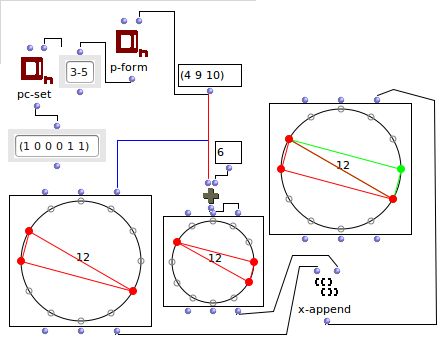
\includegraphics[scale=0.7]{OM_settheory/notas_comuns_tritono.png}
	\end{center}
	\legend{Fonte: autor }
\end{figure}

É preciso observar que para o caso do trítono a inversão é simétrica - portanto para cada trítono temos duas notas em comum. Como no exemplo acima: 10 e 4 geram as duas simétricas 4 e 10, logo conclui-se que um trítono gera duas notas em comum e assim por diante.

Interessante pensar também que o vetor de intervalos irá determinar transposições onde não existe nota nenhuma em comum. Composicionalmente isso pode ser visto como uma possibilidade de transpor a série para uma sessão totalmente distinta da anterior, criando algum discurso com estas transições.


\subsection{Simetria Transpositiva}

Na simetria transpositiva temos um padrão de intervalos que funciona como palíndromo (tem a mesma leitura da esquerda para a direita e direita para esquerda).

\begin{figure}[!h]
	\caption{\label{fig_grafico}A simetria transpositiva é obtida através de um padrão de intervalo palíndromo. }
	\begin{center}
	    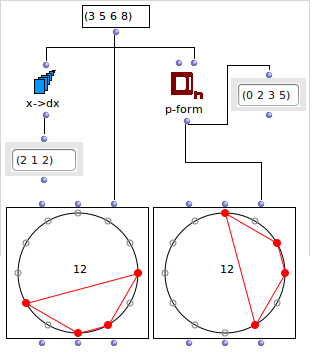
\includegraphics[scale=0.6]{OM_settheory/palindrome1.png}
	\end{center}
	\legend{Fonte: autor }
\end{figure}



\begin{figure}[!h]
	\caption{\label{fig_grafico}A forma circular é mais geral do que a numérica para a visualização do padrão de simetrias. }
	\begin{center}
	    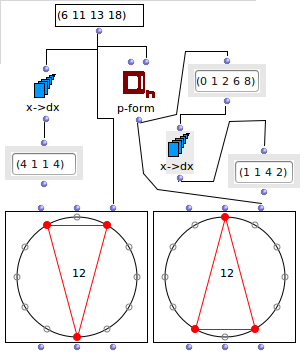
\includegraphics[scale=0.6]{OM_settheory/palindrome2.png}
	\end{center}
	\legend{Fonte: autor }
\end{figure}



\subsection{Complemento}

Útil para reconhecer e produzir contextos totalmente distintos entre si, o complemento é composto por todos intervalos que estão exclusos dos grupo, produzindo um outro grupo completamente diferente.


\begin{figure}[!h]
	\caption{\label{fig_grafico}O complemento contém todas alturas cromáticas que o conjunto original não possui. }
	\begin{center}
	    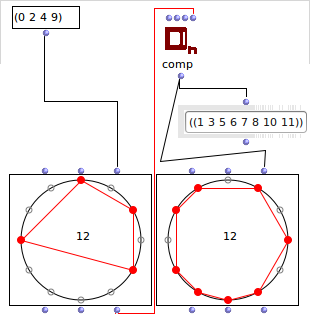
\includegraphics[scale=0.6]{OM_settheory/complemento.png}
	\end{center}
	\legend{Fonte: autor }
\end{figure}


\subsection{Relação Z entre grupos de classes de alturas}

A relação Z é uma das interessantes relações onde há uma equivalência sem que os conjuntos sejam transposições ou inversões entre si neste caso produzindo dois conjuntos que possuem os mesmos intervalos na sua constituição.


\begin{figure}[!h]
	\caption{\label{fig_grafico}Dois conjuntos Z-relacionados possuem os mesmos intervalos sem serem inversões ou transposições uns dos outros. }
	\begin{center}
	    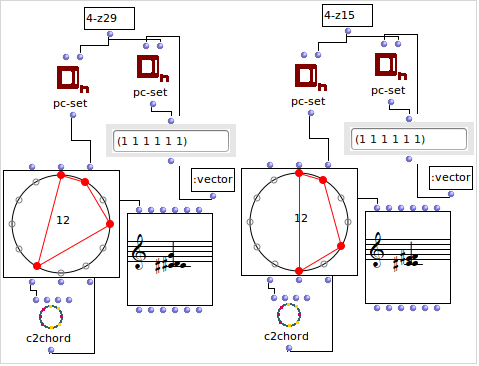
\includegraphics[scale=0.7]{OM_settheory/Z_related.png}
	\end{center}
	\legend{Fonte: autor (adaptado de exemplo do tutorial MathTools do OM) }
\end{figure}

\end{apendicesenv}
% ---
% ----------------------------------------------------------





% ----------------------------------------------------------
% Anexos
% ----------------------------------------------------------

% ---
% Inicia os anexos
% ---
%\begin{anexosenv}

% Imprime uma página indicando o início dos anexos
%\partanexos



% ---
%\chapter{Regras da Teoria Gerativa da Musica Tonal}
% ---


%\end{anexosenv}

%---------------------------------------------------------------------
% INDICE REMISSIVO
%---------------------------------------------------------------------
\phantompart
\printindex
%---------------------------------------------------------------------

\end{document}
